\chapter{Banco de dados}\label{cap:cap1}

\begin{flushright}
  \textit{
    Persistência é a irmã gêmea da excelência. \\
    Uma é a mãe da qualidade, a outra é a mãe do tempo.
  } \\
  
  \textbf{Marabel Morgan}
\end{flushright}

O armazenamento de dados é uma faceta crucial em qualquer aplicação de computador. Ele permite a captura e preservação de informações para análise futura ou para alimentar a geração de resultados esperados. Há uma ampla variedade de opções de armazenamento de dados, incluindo arquivos (texto e/ou binários), bancos de dados relacionais, sistemas NoSQL e outros tipos de soluções.

Contudo, apesar da existência de diversas formas de armazenar dados, o objetivo deste texto é demonstrar o uso de um banco de dados relacional juntamente com o NodeJS. Para tal, será utilizada a linguagem padrão de consulta, a SQL (Structured Query Language).

A linguagem de consulta SQL é um padrão amplamente utilizado em muitos sistemas de gerenciamento de banco de dados relacional (também conhecidos como SGDBs). No entanto, a implementação do SQL pode variar em relação ao padrão oficial. Essas variações normalmente não são um problema quando você trabalha apenas com uma plataforma específica de banco de dados. No entanto, quando você precisa mudar entre diferentes provedores de banco de dados ou mesmo entre versões diferentes do mesmo provedor, essas diferenças podem se tornar importantes. A mudança para sistemas não relacionais aumenta ainda mais a complexidade do problema. Portanto, é importante considerar cuidadosamente o projeto antes de decidir qual banco de dados utilizar. 

Já o banco escolhido, inicialmente, será o Postgresql. Esse SGDB, segundo seus desenvolvedores, é poderoso sistema de banco de dados objeto-relacional de código aberto com mais de 30 anos de desenvolvimento ativo que lhe rendeu uma forte reputação de confiabilidade, robustez de recursos e desempenho\footnote{Para mais detalhes, acesse: \url{https://www.postgresql.org}}. 

As notas de aula, não se preocupam com detalhes de instalação e/ou configuração, pois se acredita que, nesse momento do curso, o estudante já está capacitado para tal tarefa. Contudo, caso o leitor queira montar seu ambiente de trabalho, segue as tecnologias base que serão utilizadas nesse primeiro capítulo.

\begin{itemize}
	\item NodeJS - versão 16+
	\item Express - versão 4+
	\item Postgres - 14+ (será usado a versão online disponível em: \url{https://www.elephantsql.com})
\end{itemize}

\section{Conceitos básicos sobre Banco de dados Relacionais}

Segundo \citeonline{elmasri2005sistemas}, um banco de dados é uma coleção de dados relacionados. Os dados são fatos que podem ser gravados e que possuem um significado implícito. Por exemplo, considere nomes, números telefônicos e endereços de pessoas que você conhece. Esses dados podem ter sido escritos em uma agenda de telefones ou armazenados em um computador. Essas informações são uma coleção de dados com um significado implícito, consequentemente, um banco de dados.

Ainda, segundo os autores:

\begin{citacao}
	Um banco de dados pode ser gerado e mantido manualmente ou pode ser automatizado (computadorizado). Por exemplo, um catálogo de cartões bibliotecários é um banco de dados que oferece a possibilidade de ser criado e mantido manualmente. Um banco de dados computadorizado pode ser criado e mantido tanto por um grupo de aplicativos escritos especialmente para essa tarefa como por um sistema gerenciador de banco de dados \cite[p. 04]{elmasri2005sistemas}.
\end{citacao}

Já, um Sistema Gerenciador de Banco de dados, (SGBD) é uma coleção de programas que permite aos usuários criar e manter um banco de dados. O SGBD é, portanto, um sistema de software de propósito geral que facilita os processos de definição, construção, manipulação e compartilhamento de bancos de dados entre vários usuários e aplicações \cite{elmasri2005sistemas}. 

Assim, a base de dados e o software de gerenciamento da base de dados compõem o chamado Sistema de Base de Dados. A Figura \ref{fig:sdbd} apresenta um esquema genérico de um Sistema de Banco de Dados em sua interação com seus usuários \cite{takai2005introduccao}.

\begin{figure}[H]
	\centering
		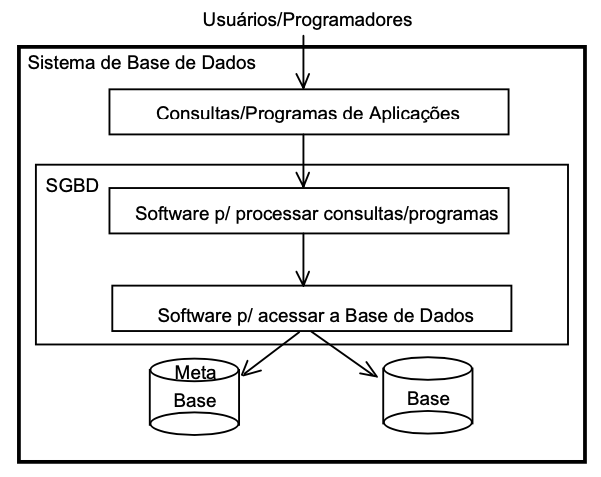
\includegraphics[scale=0.4]{imagens/sdbd.png}
	\caption{
		Sistema de Banco de Dados
		Fonte: \cite{takai2005introduccao}
	}
	\label{fig:sdbd}
\end{figure}

\subsection{Modelo Entidade-Relacionamento: Entidades e atributos}

O objeto básico que o Modelo Entidade-Relacionamento (MER) representa é a \textbf{entidade}. Uma entidade é algo do mundo real que possui uma existência independente. Uma entidade pode ser um objeto com uma existência física - uma pessoa, carro ou empregado - ou pode ser um objeto com existência conceitual - uma companhia, um trabalho ou um curso universitário. Já, cada entidade tem propriedades particulares, chamadas atributos, que a descrevem \cite{takai2005introduccao}.

\begin{figure}[H]
	\centering
	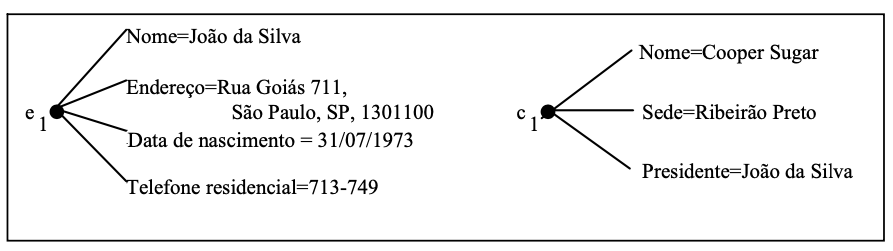
\includegraphics[scale=0.4]{imagens/entidade-atributos.png}
	\caption{
		Exemplo de entidades e seus respectivos atributos
		Fonte: \cite{takai2005introduccao}
	}
	\label{fig:entidade-atributos}
\end{figure}

Alguns atributos podem ser divididos em subpartes com significados independentes. Por exemplo, \textbf{Endereço}, como visto na Figura \ref{fig:atributos-compostos}, pode ser dividido em\textbf{ Endereço da Rua, Cidade, Estado e CEP}. Um atributo que é composto de outros atributos mais básicos é chamado \textbf{composto}. Já, atributos que não são divisíveis são chamados \textbf{simples} ou \textbf{atômicos}.

Tipos de atributos:

\begin{itemize}
	\item \textbf{Compostos}: Podem ser divididos em partes menores;
	\item \textbf{Simples}: Eles não são divisíveis;
	\item \textbf{Monovalorados}: Possuem apenas um valor;
	\item \textbf{Multivalorado}: Um ou mais valores para o mesmo;
	\item \textbf{Armazenado}: Em geral todos os atributos são armazenados;
	\item \textbf{Derivado}: Alguns atributos podem ter uma relação entre si;
	\item \textbf{Nulo}: Quando valores podem não ser aplicados.
\end{itemize}

\begin{figure}[H]
	\centering
	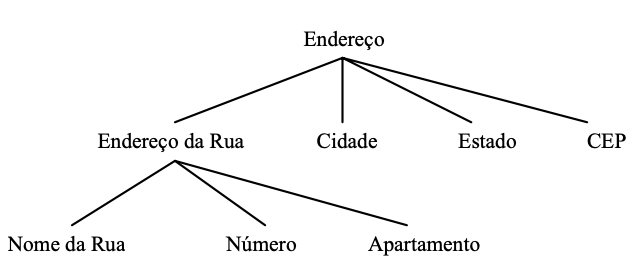
\includegraphics[scale=0.4]{imagens/atributos-compostos.png}
	\caption{
		Exemplo de atributos compostos
		Fonte: \cite{takai2005introduccao}
	}
	\label{fig:atributos-compostos}
\end{figure}

Um banco de dados inclui uma coleção de conjuntos de entidades, cada qual contendo um número de entidades do mesmo tipo. A figura abaixo mostra parte de um banco de dados que consiste em dois conjuntos de entidades: clientes e contas \cite{fundamentos2005Sanches}

\begin{figure}[H]
	\centering
	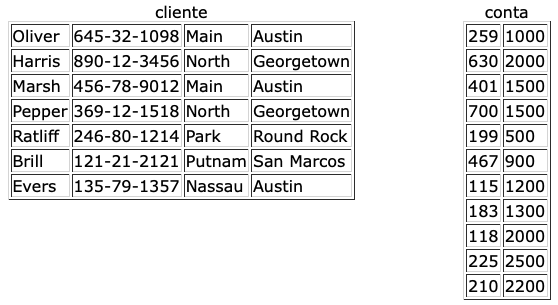
\includegraphics[scale=0.6]{imagens/tabela1.png}
	\caption{
		Conjuntos de entidades cliente e conta.
		Fonte: \cite{fundamentos2005Sanches}
	}
	\label{fig:client-conta-1}
\end{figure}

\subsection{Relacionamentos e conjunto de relacionamentos}

Um relacionamento, segundo \citeonline{fundamentos2005Sanches}, é uma associação entre diversas entidades. Por exemplo, podemos definir um relacionamento que associa o \textbf{cliente Harris} à \textbf{conta 401}. Isto especifica que Harris é um cliente com conta bancária número 401. Assim, o relacionamento ContaCliente é um exemplo de um conjunto de relacionamentos \textbf{binários} - isto é, ele envolve dois conjuntos de entidades.

\begin{figure}[H]
	\centering
	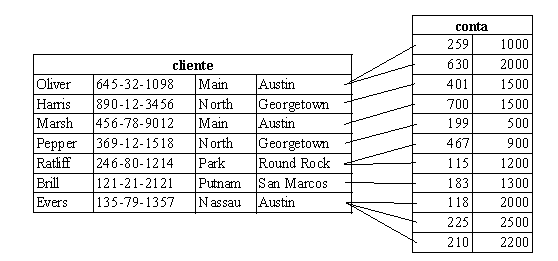
\includegraphics[scale=0.7]{imagens/relacionamento.png}
	\caption{
		Relacionamento envolvendo entidades: \textbf{Cliente} e \textbf{Conta}.
		Fonte: \cite{fundamentos2005Sanches}
	}
	\label{fig:relacionamento-1}
\end{figure}

Os relacionamentos podem ser: 

\begin{itemize}
	\item \textbf{Um-para-um}: uma entidade A está associada no máximo a uma entidade B e uma entidade B está associada no máximo a entidade de A;
	\item \textbf{Um-para-muitos}: uma entidade A está associada a qualquer número de entidades de B. Uma entidade de B, entretanto, pode estar associada no máximo a uma entidade de A;
	\item \textbf{Muitos-para-um}: uma entidade A está associada no máximo a uma entidades de B. Uma entidade de B, entretanto, pode estar associada a qualquer número de entidades de A;
	\item \textbf{Muitos-para-muitos}: uma entidade A está associada a qualquer número de entidades de B e uma entidade de B está associada a qualquer número de entidades de A.
\end{itemize}

Abaixo, na Figura \ref{fig:tipos-de-relacionamento}, pode-se visualizar as formas de relacionamento, como as entidades podem se relacionar para mais dar sentido a informação desejada.

\begin{figure}[H]
	\centering
	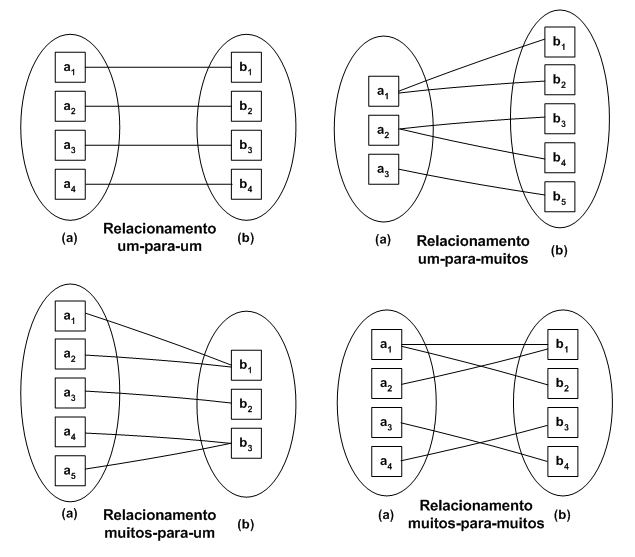
\includegraphics[scale=0.6]{imagens/relacionamentos-2.png}
	\caption{Tipos de relacionamento. Fonte: \cite{fundamentos2005Sanches}}
	\label{fig:tipos-de-relacionamento}
\end{figure}

\subsection{Linguagens de SGBD’s relacionais} 

A linguagem de SGBD's é essencialmente SQL, que no que lhe concerne é subdividido em grupos de comandos, conforme a função de cada comando.

e, resumindo,

\begin{itemize}
	\item \textbf{DDL} = Data Definition Language - Linguagem de definição de dados, possibilita a definição ou descrição dos objetos do BD.
	\item \textbf{DML} = Data Manipulation Language - Linguagem de manipulação de dados, que suporta manipulação (acesso e alteração).
	\item \textbf{DCL} = Data Control Language - Linguagem de controle de dados, possibilita a determinação das permissões que cada usuário terá sobre os objetos do BD (permissão de criação, consulta, alteração, etc.).
\end{itemize}

Para este estudo, consideraremos apenas as DML que serão utilizadas no próximo capítulo. A Linguagem de Manipulação de Dados (DML - \textbf{Data Manipulation Language}) é um conjunto de comandos que determinam quais valores estão presentes nas tabelas em qualquer momento e como serão manipulados. No SQL, por exemplo, são instruções DML: 

\begin{itemize}
	\item SELECT - consulta (seleção) 
	\item UPDATE - atualização
	\item DELETE - exclusão
	\item INSERT - inclusão
\end{itemize}

De forma simples, para ser realizada uma seleção de alguns dados no banco, pode-se fazer da seguinte forma:

\begin{lstlisting}
	select * from ENTIDADE
	select * from ENTIDADE where ATRIBUTO = VALOR DESEJADO
	select NOME_DA_COLUNA FROM ENTIDADE_1 inner join ENTIDADE_2
	ON ENTIDADE_1.coluna_nome = ENTIDADE_2.coluna_nome;
\end{lstlisting}

Existem varias formas de se fazer uma seleção, atualização, entre outros. Contudo, em nossas práticas diárias, faremos algumas delas considerando o conhecimento adquirido pelo estudante no decorrer de várias disciplinas relacionadas a Banco de dados. 

\subsection{Exercícios de fixação}

\begin{enumerate}
	\item Defina os seguintes termos: dados, informação, banco de dados, SGBD e sistema de banco de dados.
	\item Quais podem ser as diferentes categorias de usuários finais de banco de dados? Discuta as atividades principais de cada um.
	\item Cite e explique algumas vantagens do uso de Banco de dados.
	\item Quais são as categorias de linguagens de SGBD? Para que serve cada uma?
	\item Uma escola possui várias turmas. Uma turma contém vários professores na qual um professor pode lecionar aulas em mais de uma turma. Uma turma possuí sempre aulas na mesma sala, mas uma sala pode estar associada a várias turmas.
	\begin{enumerate}
		\item Liste as possíveis entidades que podem ser encontradas
		\item Liste os possíveis atributos das entidades encontradas
		\item Relacione, de forma simples, as entidades.
	\end{enumerate}
\end{enumerate}